\section{A Family of Contact Models}
\label{sec:models_family}

We present a family of models satisfying \eqref{eq:curl_tangent} and establish
conditions for convexity. Moreover, we present two novel convex approximations
of contact: Lagged and Similar.

\subsection{SAP model}

While SAP \cite{bib:castro2022unconstrained} is convex by construction, it is a
good exercise to verify our new conditions hold for this model. From
\cite{bib:castro2022unconstrained}, we know that the Hessian of the regularizer
cost
\begin{equation*}
    \mf{G} = \frac{\partial^2\ell}{\partial\mf{v}_c^2} = -\frac{\partial\bgamma}{\partial\mf{v}_c}=
    -\begin{bmatrix}
		\frac{\partial\bgamma_t}{\partial\mf{v}_t} & \frac{\partial\bgamma_t}{\partial v_n}\\
		\frac{\partial\gamma_n}{\partial\mf{v}_t}^T & \frac{\partial\gamma_n}{\partial v_n}\\
	\end{bmatrix}
\end{equation*}
is symmetric positive semi-definite and therefore SAP satisfies condition
\eqref{eq:curl_tangent}. Moreover, $\partial\bgamma_t/\partial\mf{v}_t$ is
symmetric since $\bgamma_t$ is of the isotropic form
\eqref{eq:generic_friction_model} and condition \eqref{eq:curl_normal} is met.

\subsection{Lagged Model}
\label{sec:lagged_model}

We use the model of regularized friction \eqref{eq:regularized_friction} in
which the normal impulse is \emph{lagged} to the previous time step
\begin{equation}
    \bgamma_t(\vf{v}_t)=-\mu\,f(s)\gamma_{n,0}\hat{\mf{t}}
    \label{eq:lagged_friction_model}
\end{equation}
with $s=\Vert\mf{v}_t\Vert/\varepsilon_s$, and using
\eqref{eq:generic_force_law}, $\gamma_{n,0}=\delta t f_n(\phi_0, v_{n,0})$. For a
physical model of compliance for which $\gamma_n$ is only a function of $v_n$,
condition \eqref{eq:curl_tangent} is trivially met since
\begin{eqnarray*}
    \frac{\partial\bgamma_t}{\partial v_n}=\mf{0}\\
    \frac{\partial\gamma_n}{\partial\mf{v}_t}=\mf{0}
\end{eqnarray*}

In this model, the normal impulses are still treated implicitly, with potential
$\ell_n=-N(v_n)$ and impulse $\gamma_n=n(v_n)$. The normal impulse is only
lagged in the friction model.

We verify that
\begin{equation*}
    \ell_t(\vf{v}_t) = \mu\gamma_{n0}\,\varepsilon_s\,F(\Vert\vf{v}_t\Vert/\varepsilon_s)
\end{equation*}
with $f = F'$ satisfies $\bgamma_t = -\partial\ell_t/\partial\mf{v}_t$. The
contact potential is separable as the sum of normal and friction contributions
\begin{equation*}
    \ell(\vf{v}_c) = \ell_t(\vf{v}_t) + \ell_n(v_n).
\end{equation*}

The Hessian of $\ell_t$ is given by
\begin{eqnarray*}
    \frac{\partial^2\ell_t}{\partial\vf{v}_t^2}&=&-\frac{\partial\bgamma_t}{\partial\vf{v}_t}\nonumber\\
    &=&\mu\gamma_{n0}\left[\frac{f'(s)}{\varepsilon_s}\mf{P}(\hat{\vf{t}})+\frac{f(s)}{\Vert\vf{v}_t\Vert}\mf{P}^\perp(\hat{\vf{t}})\right].
\end{eqnarray*}

With a non-decreasing $f$ , $F$ is convex, and the Hessian of $\ell_t$ is the
positive linear combination of two projection matrices. Therefore, $\ell_t$ is
twice differentiable and convex. Thus the Hessian
\begin{equation*}
    \frac{\partial^2\ell}{\partial\mf{v}_c^2} = -\frac{\partial\bgamma}{\partial\mf{v}_c}=
    \begin{bmatrix}
		-\frac{\partial\bgamma_t}{\partial\mf{v}_t} & \vf{0}\\
		\vf{0}^T & -\frac{\partial\gamma_n}{\partial v_n}\\
	\end{bmatrix}
\end{equation*}
is positive definite for physics-based model that satisfy
\eqref{eq:normal_sufficient_conditions}.

As in Section \ref{sec:regularized_friction}, the judicious choice
$F(s)=\sqrt{s^2+1}-1$ leads to expressions of the cost, gradient, and Hessian
involving soft norms (Appendix \ref{sec:soft_norms}) which are twice
differentiable and convex, even at $\vf{v}_t=\vf{0}$
\begin{eqnarray*}
    \ell_t(\vf{v}_t) &= \mu\gamma_{n0}\,\Vert\vf{v}_t\Vert_s,\nonumber\\
    \bgamma_t&=-\mu\,\gamma_{n,0}\hat{\mf{t}}_s,\nonumber\\
    \frac{\partial^2\ell_t}{\partial\vf{v}_t^2}&=\mu\gamma_{n0}\frac{\mf{P}^\perp(\hat{\vf{t}}_{s})}{\Vert\vf{v}_t\Vert_s+\varepsilon_s}.
\end{eqnarray*}

\subsection{Similar Model}
\label{sec:similar_model}

Similarity solutions to partial differential equations (PDEs) are solutions which depend on certain groupings of
independent variables rather than each variable individually. In particular,
self-similar solutions arise when the problem lacks a characteristic time or
length scale. The Blasius solution to Prandtl's boundary layer equations in
fluid mechanics is a well-known and celebrated example.

 Motivated by the algebraic form of SAP impulses
\cite{bib:castro2022unconstrained}, we propose the grouping of variables $z =
v_n-\mu\Vert\vf{v}_t\Vert$. Furthermore, we generalize this grouping to
\begin{equation}
    z = v_n-\mu \varepsilon_sF(s),
    \label{eq:similar_grouping}
\end{equation}
where as in Section \ref{sec:lagged_model}, $\mu \varepsilon_sF(s)$ simplifies
to $\mu\Vert\vf{v}_t\Vert_s$ when $F(s)=\sqrt{s^2+1}-1$. Note the consistency of
units in \eqref{eq:similar_grouping}, an inportant aspect of similar solutions.
With this grouping, we propose the \emph{similar} solution
\begin{eqnarray}
    \gamma_n(\Vert\vf{v}_t\Vert,v_n) &=& n(z),\nonumber\\
    \bgamma_t(\Vert\vf{v}_t\Vert,v_n) &=&
    -\mu\,f(s)\,\gamma_n(\Vert\vf{v}_t\Vert,v_n)\,\hat{\vf{t}}.
    \label{eq:impulses_convexified}
\end{eqnarray}

Unlike the Lagged model, the Similar model strongly couples friction and normal
components. However, this introduces a dependency of the normal component on
slip speed, an artifact we quantify in the following sections.

Differentiation of \eqref{eq:impulses_convexified} leads to
\begin{eqnarray*}
    \frac{\partial\bgamma_t}{\partial
    v_n}=\frac{\partial\gamma_n}{\partial\mf{v}_t}=-\mu\,f(s)\,n'(z)\,\hat{\vf{t}},
\end{eqnarray*}
which confirms condition \eqref{eq:curl_tangent}. To find the potential, we
start from the normal component of the impulse
\begin{equation*}
    \gamma_n(\Vert\vf{v}_t\Vert,v_n) = n(z) = -\frac{\partial\ell}{\partial v_n},
\end{equation*}
and integrate on $v_n$ to obtain
\begin{equation*}
    \ell(\vf{v}_t,v_n) = -N(z) + G(\vf{v}_t),
\end{equation*}
where $G(\vf{v}_t)$ is an arbitrary function of $\vf{v}_t$. Taking the
derivative with respect to $\vf{v}_t$ results in
\begin{equation*}
    \frac{\partial\ell}{\partial\vf{v}_t}=\mu\,n(z)\,f(s)\hat{\vf{t}} + \frac{\partial G}{\partial\vf{v}_t}.
\end{equation*}

Comparing this last equation with \eqref{eq:impulses_convexified} reveals that we can
set $G=0$ and obtain
\begin{equation}
    \ell(\Vert\vf{v}_t\Vert,v_n) = -N(z),
    \label{eq:similar_potential}
\end{equation}
as the desired potential function.

The Hessian of this potential is
\begin{eqnarray*}
    &&\frac{\partial^2\ell}{\partial\vf{v}_c^2}=-\frac{\partial\bgamma}{\partial\vf{v}_c}=\\
    &&\begin{split} =&\mu\left[
        \left(\frac{f'(s)n(z)}{\varepsilon_s}-n'(z)f^2(s)\right)\mf{P}(\hat{\vf{t}})\right.\\
    &+\left.\frac{f(s)n(z)}{\Vert\vf{v}_t\Vert}\mf{P}^\perp(\hat{\vf{t}})\right].
    \end{split}\nonumber
\end{eqnarray*}

For a convex potential $\ell_n$ we have $n'=N''=-\ell_n'' \leq 0$. With $f(s)$
non-decreasing as in the lagged model, $f'\ge 0$. The Hessian
$\partial^2\ell/\partial\vf{v}_c^2$ is the linear combination with positive
coefficients of symmetric positive semi-definite projection matrices. Therefore,
the Hessian is symmetric positive semi-definite, and the potential is convex. As
before, the choice $F(s)=\sqrt{s^2+1}-1$ leads to continuously differentiable
expressions in terms of soft norms (Appendix \ref{sec:soft_norms}), with no
singularity at $\vf{v}_t=\vf{0}$.

Our \emph{Similar} model closely relates to the primal formulation
\cite{bib:mazhar2014,bib:castro2022unconstrained} of Anitescu's convex
approximation \cite{bib:anitescu2006}. Following
\cite{bib:castro2022unconstrained} we define the velocity $\vf{g} = \vf{v}_c -
\hat{\vf{v}}_c$, with $\hat{\vf{v}}_c=[0, 0, \hat{v}]^T$ and the \emph{breaking
velocity} from \eqref{eq:breaking_velocity}. Using this definition, we express $z$
as $z = g_n-\mu \varepsilon_sF(\Vert\vf{g}_t\Vert/\varepsilon_s) + \hat{v}$. We
notice that $\ell(z)$ is constant (no contact) for $z\ge\hat{v}$. In terms of
$\vf{g}$, this is equivalent to $g_n-\mu
\varepsilon_sF(\Vert\vf{g}_t\Vert/\varepsilon_s) \ge 0$. The graph of $g_n=\mu
\varepsilon_sF(\Vert\vf{g}_t\Vert/\varepsilon_s)$ defines the boundary of the
stick-slip transition, and therefore when $F(s)$ is convex, its epigraph (the
set of points above its graph), corresponds to a convex region (not necessarily
a cone as in previous work). This is illustrated in Fig. \ref{fig:dual_cone}. In
this plot, contour levels of $\ell(\Vert\vf{g}_t\Vert,g_n)$ correspond to lines
of constant $z$, which by definition are perpendicular to the gradient
$\partial\ell/\partial\mf{v}_c$. We see that the role of the potential $\ell$ is
to penalize $\vf{g}$ when it lies outside the epigraph of $g_n=\mu
\varepsilon_sF(\Vert\vf{g}_t\Vert/\varepsilon_s)$.

Consider $F(s)=\sqrt{s^2+1}-1$, for which $g_n = \mu \Vert\vf{g}_t\Vert_s$. The
epigraph of this function is an approximation to the dual $\mathcal{F}^*$ of the
friction cone $\mathcal{F}$, Fig. \ref{fig:dual_cone}. This approximation is
$\mathcal{F}^*$ in the limit $\varepsilon_s\rightarrow 0$. Moreover, in the
limit to rigid contact, $\ell$ enforces $\vf{g} \in \mathcal{F}^*$, which
corresponds to the cone constraint in the primal formulation
\cite{bib:mazhar2014,bib:castro2022unconstrained}.

\begin{figure}[!h]
    \centering
    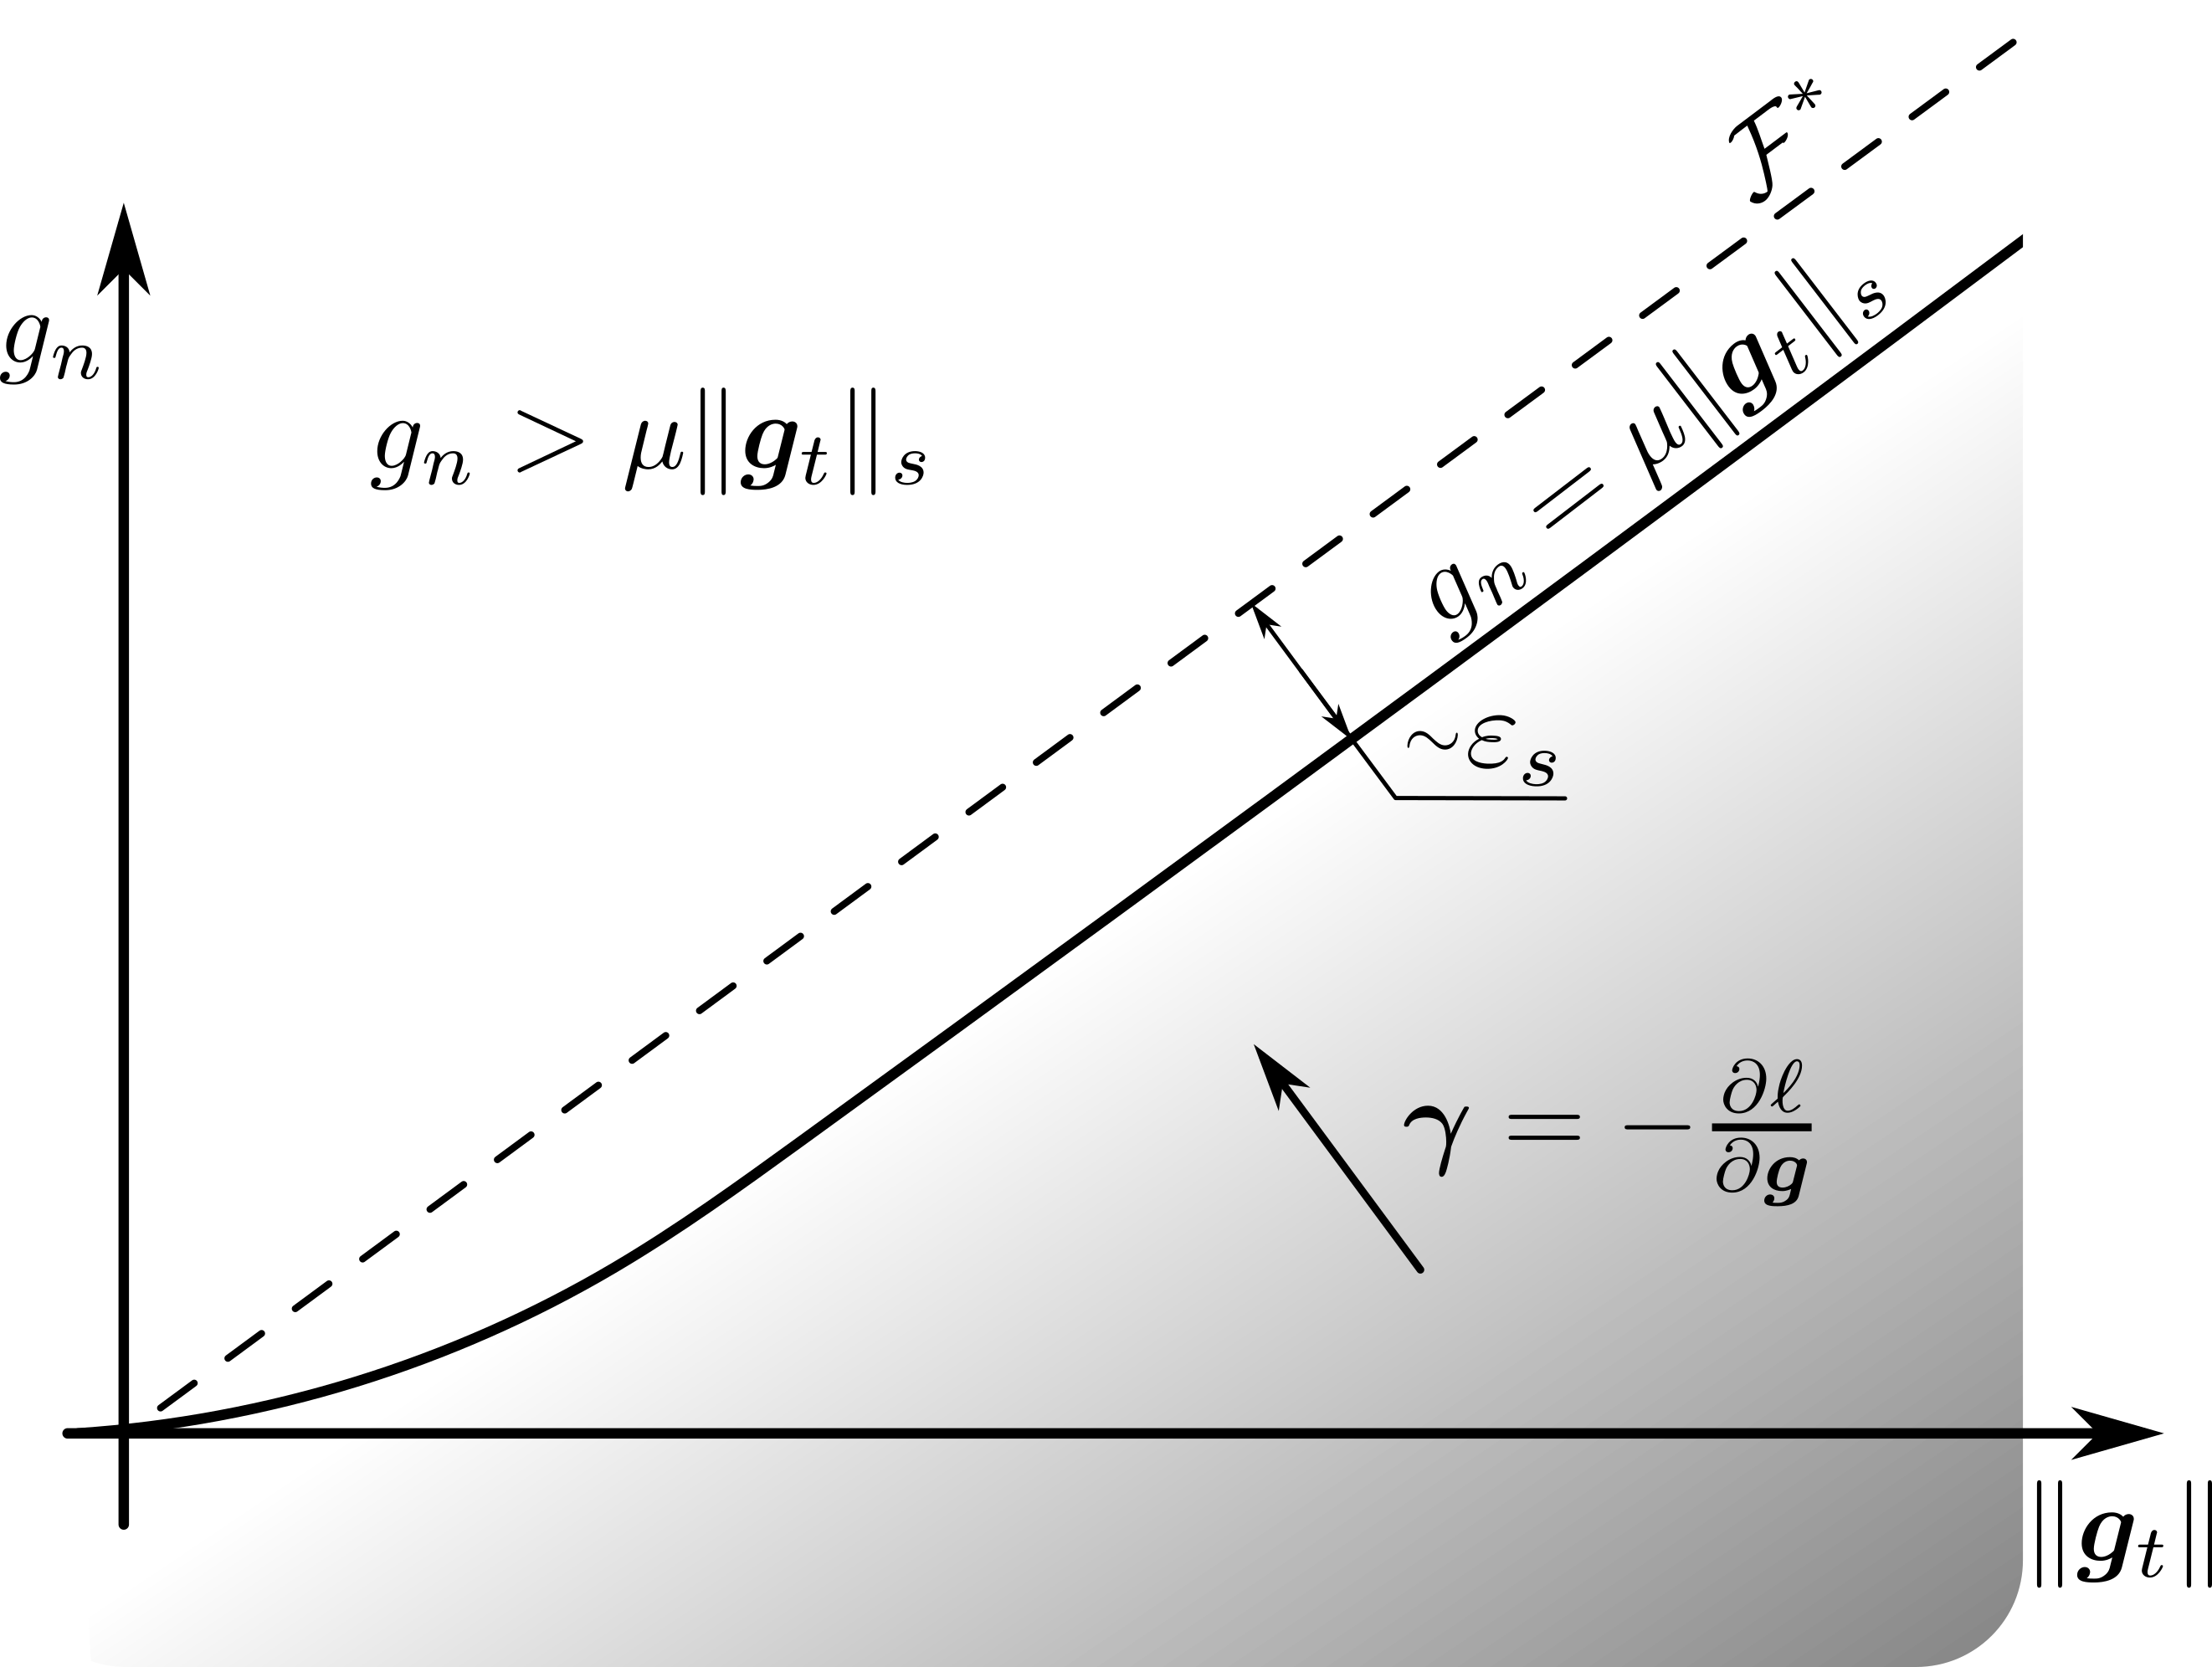
\includegraphics[width=0.6\columnwidth]{figures/similar_cones.png}
    \caption{The \emph{Similar} model penalizes $\vf{g}$ when it lies outside
    the region $g_n \ge \mu \varepsilon_sF(\Vert\vf{g}_t\Vert/\varepsilon_s)$.
    With $F(s)=\sqrt{s^2+1}-1$ and $\varepsilon_s\rightarrow 0$, the model
    enforces $\vf{g} \in \mathcal{F}^*$ in the limit to rigid contact,
    consistent with the primal formulations in
    \cite{bib:mazhar2014,bib:castro2022unconstrained}.}
    \label{fig:dual_cone}
\end{figure}

